\chapter{Implementierung}

Dieses Kapitel beschreibt die Implementierung von Runtime Node und Master und vergleicht die Scheduling-Methoden.

\section{Implementierung Runtime Node}

Die Runtime Node Komponente wird auf Fahrzeugsteuergeräten ausgeführt, deren Anforderungen bei der Implementierung berücksichtigt werden müssen. Die Wahl der für die Implementierung verwendeten Programmiersprache sollte so erfolgen, dass eine möglichst hohe Kompatibilität mit den benötigten Softwarebibliotheken besteht und eine Kompilierbarkeit auf möglichst vielen Hardwarearchitekturen gegeben ist. In der \autoref{Methode Softwareplattform und Scheduling} wurde festgelegt, dass die Runtime Node Linux-Kernel-basierte Betriebssysteme voraussetzt. Der Kernel dieser Systeme ist in der Programmiersprache C implementiert. Im Vergleich zu anderen weit verbreiteten Programmiersprachen wie C++, Java, Python oder Rust ist C näher an der Hardware. Gängige C-Compiler wie GCC, Clang/LLVM oder MSVC unterstützen die meisten Hardwarearchitekturen. Für spezialisierte Plattformen im Embedded-Bereich existiert ebenfalls sehr häufig eine C-Toolchain. Aus diesem Grund eignet sich die Programmiersprache C gut als Sprache für die Implementierung des Runtime Node. Im Folgenden werden die konkreten Vorgehensweisen zur Implementierung der Softwarekomponenten des Runtime Node beschrieben.

\subsection{Implementierung der Container Management}

Mit dem Container Management werden isolierte Umgebungen für externe Anwendungen erstellt und verwaltet. Dabei kommt die Containerisierung als Isolierungsmethode zum Einsatz. Bei dieser Methode werden Linux-Kernel-Funktionen genutzt, um eine isolierte Laufzeitumgebung zu erstellen, die als Container bezeichnet wird. Das Container Management implementiert vier Hauptfunktionen:

\begin{itemize}
    \item Container erstellen
    \item Container starten
    \item Container stoppen
    \item Container löschen
\end{itemize}

Die Erstellung eines Containers wird durch einen entsprechenden Befehl ausgelöst. In diesem muss ein Containername definiert werden, der anschließend intern zur Identifikation des Containers verwendet wird. Zunächst wird überprüft ob ein Container mit dem gleichen Namen bereits angelegt wurde. Wird der Name bereits verwendet, wird kein neuer Container erstellt und eine entsprechende Fehlermeldung an den Runtime Master kommuniziert. Existiert kein Container mit dem gleichen Namen, wird ein Ordner für den neu erstellten Container angelegt. Dieser dient als Wurzelverzeichnis für die Applikation im Container. Der Runtime Node kann eine Standardvorlage für ein Wurzelverzeichnis bereitstellen und dessen Inhalt in jeden Containerordner kopieren. Dies kann beispielweise das Wurzelverzeichnis einer Linux-Distribution beinhalten, damit die Applikationen die Standardbibliotheken und Werkzeuge eines Betriebssystems direkt nutzen können. Runtime Master kann nach Erstellung des Containers sowohl Applikationen als auch Softwarebibliotheken in den Containerordner über das Kommunikationsinterface übertragen. 

Die Isolierung der Applikationen erfolgt über Linux-Kerne spezifische Funktionen. Für Unix-basierte Betriebssysteme wie Linux wurde der \gls{POSIX}-Standard entwickelt, um die Kompatibilität von Software zu erhöhen, die auf Betriebssystemfunktionen zugreift. Er definiert eine einheitliche \gls{API} für Kommandozeilen- und Shell-Funktionalität. Die \gls{API} besteht aus C Funktionen, die in der implementierten Software über die die entsprechenden header Dateien verwendet werden können.  Um die Kompatibilitätsanforderungen zu erfüllen, verwendet die Runtime Node Komponente, sofern möglich, die \gls{POSIX} \gls{API} Funktionen zur Isolierung von Anwendungen. 

Ein Container wird gestartet, indem eine der darin vorhandenen Applikationen ausgeführt wird. Ein Container kann mehrere Applikationen beinhalten, allerdings kann der Runtime-Master aktuell nur eine Applikation pro Container starten. Ein Startbefehl für einen Container definiert dessen Namen sowie den Namen der zu startenden Applikation. Zunächst wird im Runtime-Node überprüft, ob ein Container mit dem im Startbefehl angegebenen Namen existiert. Wenn diese Voraussetzung erfüllt ist, wird überprüft, ob eine Applikationsdatei mit dem angegebenen Namen im Container vorhanden ist. Sind beide Voraussetzungen erfüllt, werden die Isolierung und das Starten der Applikationsfunktion vorbereitet. Mit der \gls{POSIX} Funktion \enquote{clone} wird eine als Parameter vorgegebene Funktion als neuer Prozess erstellt, der in den nächsten Schritten vom Betriebssystem isoliert wird. Diese \enquote{clone} Funktion unterstützt die Isolierung mittels Namespaces, indem die entsprechenden Unshare Flags, die im \autoref{Software Virtualisierung/Container} näher beschrieben wurden, als Parameter mitgegeben werden können. Die als Funktionsparameter übergeben Funktion wird also durch \enquote{clone} als neuer Prozess mit den vorgegebenen Isolierungsmaßnahmen ausgeführt. Die folgenden Unshare Flags werden verwendet:

\begin{itemize}
    \item CLONE\_NEWNS: Mount Namespace Unshare Flag
    \item CLONE\_NEWPID: PID Namespace Unshare Flag
    \item CLONE\_NEWUTS: IPC Namespace Unsahre Flag
    \item CLONE\_NEWNET: Network Namespace Unshare Flag
\end{itemize}

Der von der Funktion \enquote{clone} gestartete Prozess führt die Pivot-Root-Routine aus, um die Zugriffsrechte des Prozesses auf den Ordnerinhalt des Containers einzuschränken. Hierzu muss der Ordner des Containers ein Mount-Punkt des Prozesses werden. Die Systemfunktion \enquote{mount} fügt den als Parameter übergebenen Pfad als Mount-Punkt dem aktuellen Prozess hinzu. Da Pivot Root über keine \gls{POSIX}-standardisierte Wrapper-Funktion verfügt, muss es über die \enquote{syscall}-Funktion implementiert werden. Diese wird über die C-Softwarebibliothek glibc bereitgestellt, die in den meisten Linux-Distributionen enthalten ist. Abschließend wird der Prozess mit der \gls{POSIX}-Funktion \enquote{execve} durch den extern geladenen Applikation ersetzt.  Diese Applikationen werden mit allen zuvor angewendeten Isolierungsmaßnahmen im Container ausgeführt. Runtime Node erzeugt eine neue cgroup für den Prozess, sodass sowohl Systemressourcen nach Bedarf eingeschränkt werden können als auch die weiteren Prozesse, die von diesem Host-Prozess erzeugt werden, eindeutig zugeordnet werden können. Das erfolgreiche Starten der Applikation wird an den Runtime Master zurückgemeldet. 

Ein Container kann durch einen externen Befehl mit dem Namen des zu stoppenden Containers gestoppt werden. Existiert der Container mit dem Namen und wird aktuell eine Applikation ausgeführt, werden alle Prozesse im Container beendet. Hierzu genügt es, den ursprünglichen Host-Prozess zu beenden, da dieser durch die Isolierung die PID 1 erhalten hat. PID 1 wird unter Unix-Systemen als Initialisierungsprozess behandelt. Wird dieser Prozess beendet, werden alle von diesem Prozess gestarteten Prozesse ebenfalls beendet.

Container können durch den Befehl Container löschen entfernt werden. Im Befehl muss der Name des Containers angegeben werden. Existiert ein Container mit dem angegebenen Namen im Runtime-Node und führt dieser aktuell eine Anwendung aus, so wird er gestoppt und anschließend der Containerordner inklusive aller extern geladenen Dateien gelöscht.

\subsection{Implementierung Befehlsverarbeitung}
\label{Implementierung Befehlsverarbeitung}

Die Befehlsverarbeitung empfängt \gls{JSON} Nachrichten von der Kommunikationsschnittstelle, wertet sie aus und führt die entsprechenden Funktionen im Container Management Modul aus. Die \gls{JSON} Nachrichten werden über den Kommunikationssockel zwischen Node und Kommunikationsschnittstelle ausgetauscht. Zum Parsen und Erstellen von \gls{JSON} wird die Softwarebibliothek cJSON verwendet.  cJSON bietet Hilfsfunktionen für die Erzeugung und das Auslesen von \gls{JSON} Daten. Der Benutzer kann mit Hilfe dieser Funktionen \gls{JSON} Strukturen selber erstellen, sowie Parsing Funktionen für definierte Strukturen implementieren. Mit Hilfe von cJSON werden Inhalte der \gls{JSON} Nachrichten in eine interne Struktur hineinkopiert und ausgewertet. Die Befehlsnachrichten sind nach dem im \autoref{JSON command} gezeigten Format definiert. Der Inhalt des \enquote{Action} Feldes wird mit den bekannten Aktionen verglichen. 

\begin{figure}[htbp]
	\centering
	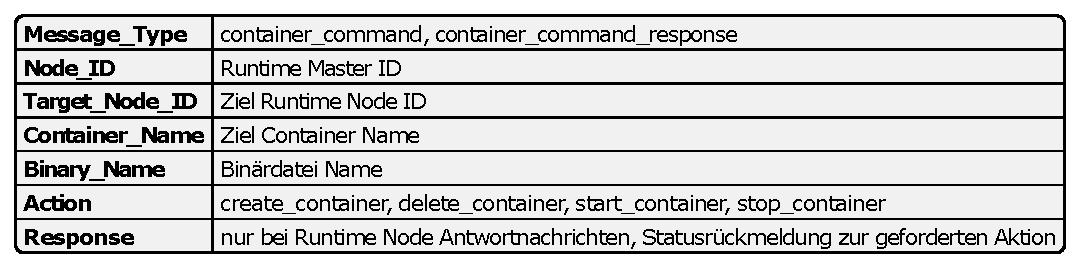
\includegraphics[width=0.9\textwidth]{./content/graphics/commandJSON.pdf}
	\caption{JSON Struktur der Befehlsübertragung}
	\label{JSON command}
\end{figure}

Bei der Auswertung eines Befehls wird zuerst überprüft ob das Feld \enquote{Target\_Node\_ID} mit dem ID des jeweiligen Runtime Nodes identisch ist. Befehle mit abweichendem ID werden ignoriert. Im nächsten Schritt wird das Feld \enquote{Action} mit den verfügbaren, implementierten Aktionen verglichen. Bei Übereinstimmung wird die entsprechende Funktion im \enquote{Container Management} mit den Parametern aus dem empfangenen Befehl aufgerufen. Unbekannte Befehle werden ignoriert.

Die Befehlsverarbeitung überträgt auch periodisch eine Node Status Meldung namens \enquote{Node\_Info}. Diese Meldung wird von jedem Runtime Node an den Runtime Master übertragen und enthält Informationen über die Rechenkapazitäten des Nodes sowie über die aktuell laufenden Applikationen. Die Struktur der Nachricht ist in der \autoref{JSON info} dargestellt.

\begin{sidewaysfigure}[htbp]
	\centering
	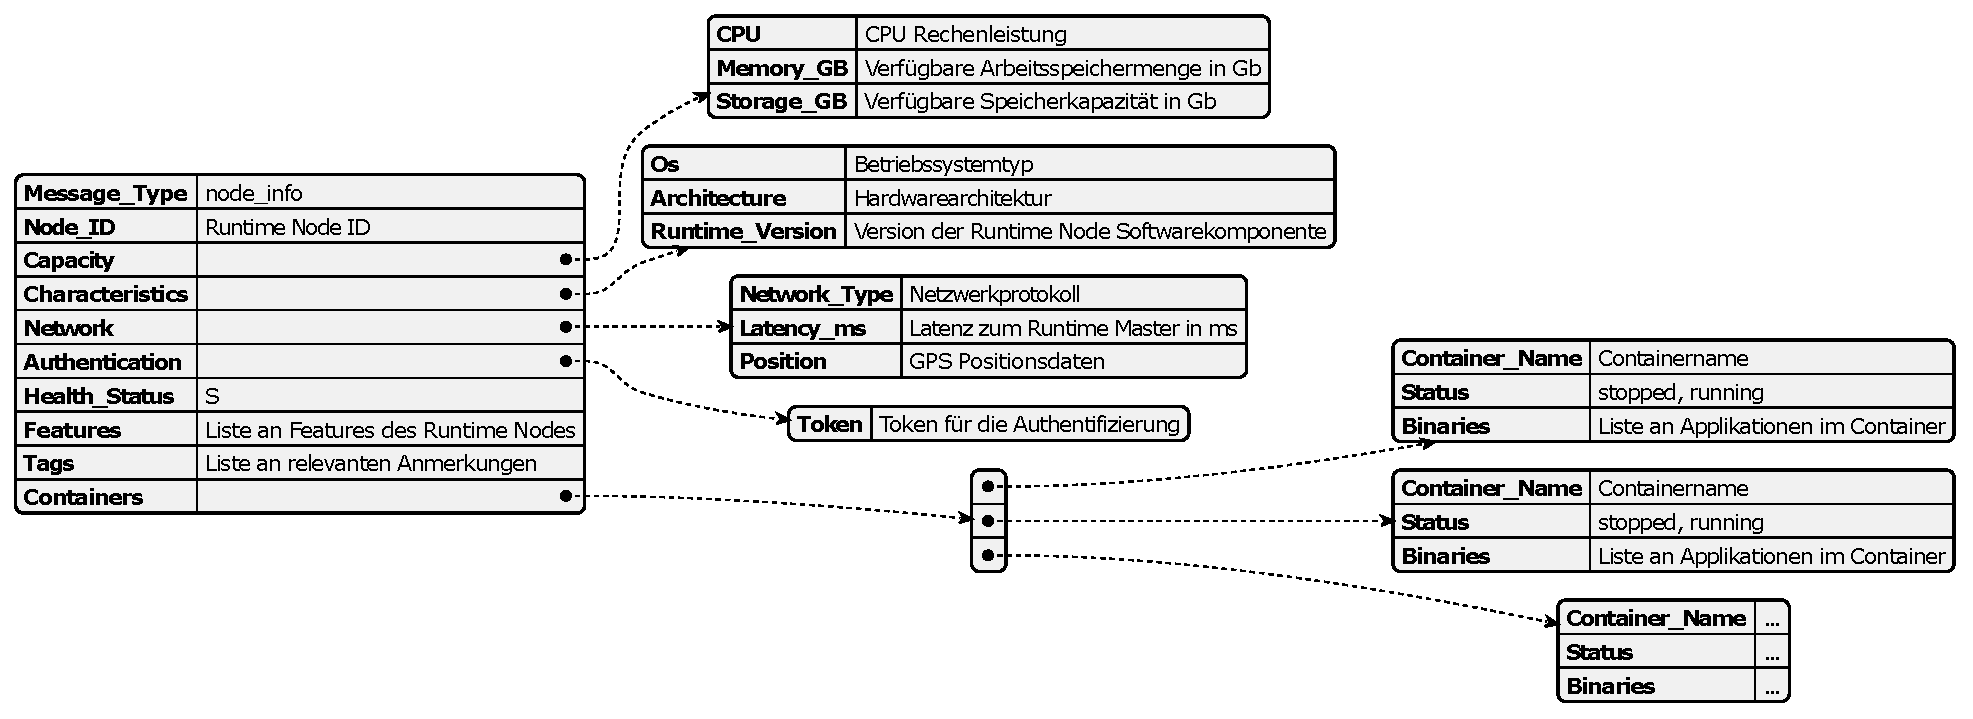
\includegraphics[width=\textwidth]{./content/graphics/infoJSON.pdf}
	\caption{JSON Struktur der Runtime Node Infonachricht}
	\label{JSON info}
\end{sidewaysfigure}

Mithilfe dieser Informationen kann der Runtime Master Scheduling Entscheidungen treffen und die Verfügbarkeit der Runtime Nodes überwachen.

\subsection{Implementierung des Ladens externer Applikationen}
\label{Laden extene Applikationen Node}

Damit extern bereitgestellte Applikationen auf den Steuergeräten des Runtime Node ausgeführt werden können, müssen die entsprechenden Dateien auf das jeweilige Steuergerät geladen werden. Für die prototypische Implementierung wurde dasselbe Kommunikationskonzept für die Übertragung von Dateien verwendet wie für die Übertragung von Befehlen und Statusmeldungen. Die Dateien werden in vorkompilierte Form im Binärformat übertragen. Die Kommunikationsschnittstelle nutzt \gls{JSON}. Nachrichten für den Informationsaustausch. Für die Übertragung wird die folgende JSON-Struktur verwendet:

\begin{figure}[htbp]
	\centering
	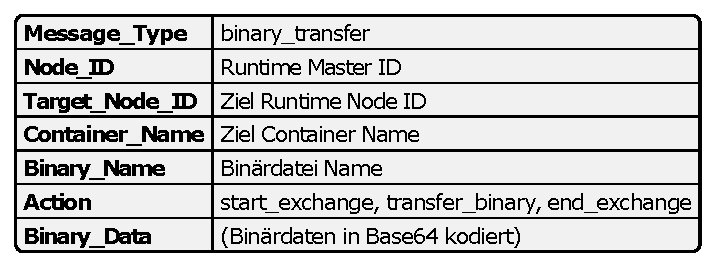
\includegraphics[width=0.6\textwidth]{./content/graphics/binaryJSON.pdf}
	\caption{JSON Struktur der Binärübertrungsnachricht}
	\label{JSON binary}
\end{figure}

\gls{JSON} Nachrichten sind charakterbasiert (in der Regel UTF-8). Die Übertragung von Binärdaten im Rohformat ist nicht möglich. Binärwerte können in \gls{JSON} nur als Zeichen dargestellt werden. Eine binäre 1 würde in diesem Fall beispielsweise mit dem Zeichen 1 dargestellt werden. Diese Methode ist sehr ineffizient, da die Darstellung von einem Bit Information acht Bits benötigt. Für Anwendungen, in denen Binärdaten in textbasierten Formaten übertragen werden müssen, wurden Binär-zu-Text-Konvertierungsschemen entwickelt. In der Implementierung wurde das Base64-Schema verwendet, das im World Wide Web weit verbreitet ist, beispielsweise für die Dateiübertragung in HTML, CSS und E-Mail-Anhängen. Base64 nimmt sechs Binärwerte und repräsentiert sie mit einem von 64 Characterzeichen. Um die Kompatibilität zu erhöhen, nutzt Base64 nur ein Basisset von \gls{ASCII} Zeichen, die von den meisten Anwendungen unterstützt werden. Dadurch wird eine möglichst hohe Portierbarkeit erreicht. Insgesamt werden mit dieser Methode sechs Binärzeichen mit einem 8-Bit-Zeichen kodiert. Die übertragene Datenmenge ist somit um 33\% höher als bei der Übertragung von binären Rohdaten. 

Die Übertragungslogik ist als State Machine implementiert. Eine Dateiübertragung kann mit der in JSON dargestellten Nachricht gestartet werden, wenn das Feld \enquote{Action} den Inhalt \enquote{start\_exchange} enthält. Wenn im Feld \enquote{Binary\_Name} kein Name einer bereits existierenden Datei angegeben ist, wird eine neue Datei mit dem definierten Namen angelegt. Eine Bestätigung über das erfolgreiche Anlegen der Datei bzw. eine Fehlermeldung wird an den Runtime Master zurückgesendet. Nach einer erfolgreichen Bestätigung beginnt Runtime Master damit, die Binärdaten der Datei zu übertragen. Die Binärdaten werden Base64 kodiert im Feld \enquote{Binary\_Data} übertragen. Dieses Feld hat eine Größe von 3.076 Bytes. Durch die Base64-Kodierung sind davon allerdings nur 2.307 Bytes Nutzdaten. In der Praxis muss eine Datei in der Regel auf mehrere Pakete aufgeteilt werden. Während der Übertragung werden die empfangenen Daten dekodiert und in die erstellte Datei geschrieben. Wurden alle empfangenen Bytes erfolgreich in die Datei geschrieben, wird eine Statusmeldung an den Runtime-Master gesendet. Wurde die Datei vollständig übertragen, wird im \enquote{Action}-Feld der Inhalt \enquote{end\_exchange} gesendet. Dies signalisiert dem Runtime-Node, dass die aktuelle Datei vollständig übertragen wurde. 

\section{Implementierung der Kommunikationsschnittstelle}

Die Kommunikationsschnittstelle ist ein eigenes Softwaremodul, das ein Publish/Subscribe-Protokoll über das Netzwerk verwendet und eine sockelbasierte Schnittstelle mit JSON zu den Softwarekomponenten hin nutzt. Im \autoref{Kommunikation zwischen Fahrzeugen und Runtime Master} wurde das Kommunikationsprotokoll Publish/Subscribe und die konkrete Implementierung \gls{DDS} ausgewählt. Die Hauptaufgabe der Kommunikationsschnittstelle ist die Konvertierung zwischen \gls{DDS} und \gls{JSON} Nachrichten. Sowohl für \gls{JSON} als auch für \gls{DDS} werden Softwarebibliotheken für die Erstellung und das Versenden sowie das Auslesen von empfangenen Nachrichten verwendet. Das Kommunikationsmodul muss folglich die Nachrichtenstrukturen und die nötigen Parsing Funktionen mit den verwendeten Bibliotheken implementieren und die Daten zwischen den Strukturen konvertieren. 

In der prototypischen Umsetzung wird die \gls{DDS} Bibliothek von der Firma eProsima verwendet. C++ kann als eine Erweiterung von C betrachtet werden. C-Code ist in der Regel auch in einer C++-Umgebung lauffähig, sodass C- und C++-Code einfach in einem Projekt kombiniert werden können. eProsima Fast DDS ist eine weit verbreitete Implementierung, die auch in \gls{ROS} 2 verwendet wird. Das Kommunikationsmodul selbst wurde ebenfalls hauptsächlich in C++ implementiert, um eine einfachere Integration mit der \gls{DDS} Bibliothek zu ermöglichen. 

Die Erstellung und Auslesen von \gls{JSON} Daten wurde mit Hilfe der Softwarebibliothek cJSON implementiert. cJSON wurde in der Programmiersprache C implementiert, so dass es auch in C++ Projekte leicht integrierbar ist. 

Beim Start verbindet sich die Kommunikationsschnittstelle mit dem Kommunikationssockel von Runtime Node oder Runtime Master und startet die konfigurierten \gls{DDS} Publisher und -Subscriber. Wird eine Nachricht über einen \gls{DDS} Subscriber empfangen, werden die Daten der Nachricht in eine interne Datenstruktur kopiert. Aus dieser Struktur wird mithilfe von cJSON die entsprechende \gls{JSON} Nachricht für den Runtime Master oder den Runtime Node erstellt und über den Kommunikationssockel versendet. Umgekehrt werden aus empfangenen \gls{JSON} Nachrichten die Daten ebenfalls in die interne Datenstruktur kopiert und aus den Daten die entsprechende \gls{DDS} Nachricht mit dem dazugehörigen \gls{DDS} Publisher versendet. Das Modul ist so implementiert, dass es sowohl für den Runtime Node als auch für den Runtime Master einsetzbar ist. Dadurch müssen nicht mehrere Varianten gepflegt werden.

\section{Implementierung Runtime Master}

Die Komponente Runtime Master ist für die Verwaltung der Runtime Nodes zuständig. Sie wird nicht auf Fahrzeugsteuergeräten, sondern einmalig pro Netzwerk auf einem zentralen Server ausgeführt. Da in der Informationstechnik hauptsächlich die x86-Architektur verwendet wird, ist die Portierbarkeit auf verschiedene Hardwarearchitekturen bei dieser Komponente nicht relevant. Bei der Auswahl der Programmiersprache bestehen daher weniger Einschränkungen. Für diese Komponente wurde eine Programmiersprache ausgewählt, die eine möglichst einfache und effiziente Implementierung ermöglicht. Die Programmiersprache Go (auch Golang genannt) wurde von Google entwickelt, um die Produktivität bei der Softwareentwicklung für Maschinen mit mehreren CPU-Kernen sowie für vernetzte Maschinen zu steigern. Die Syntax von Go ähnelt der von C, bietet jedoch erweiterte Funktionalitäten wie Goroutines, die die Erzeugung und das Scheduling von Threads vereinfachen, sowie Standardbibliotheken, die beispielsweise gängige Netzwerkprotokolle implementieren. Aus diesen Gründen wurde diese Sprache für die Implementierung der Runtime Node Komponente verwendet. 

\subsection{Implementierung Node Datenbank}

Die Node Datenbank speichert die Informationen über die Runtime Nodes, die sich aktuell im selben Netzwerk befinden. Diese Informationen werden über die im \autoref{Implementierung Befehlsverarbeitung} vorgestellten \enquote{Node Info} Nachrichten der Runtime Nodes übertragen. Die Datenbank beinhaltet alle Informationen aus den \enquote{Node Info} Nachrichten, zusätzlich wird festgehalten wann die letzte \enquote{Node Info} Nachricht empfangen wurde und ob dies im konfigurierten Zeitraum war. In der prototypischen Implementierung ist die Datenbank als interne Datenstruktur umgesetzt. Diese Methode speichert alle Einträge im Arbeitsspeicher des Systems, auf dem Runtime Master ausgeführt wird. Je nach Objektgröße können 100.000 Einträge problemlos im Arbeitsspeicher gehalten werden. Diese sind jedoch nicht persistent, da die Datenstruktur nach Beenden der Applikation gelöscht wird. Für größere Netzwerke mit vielen Teilnehmern und persistenten Daten ist es sinnvoll auf eine Datenbankimplementierung zurückzugreifen. Datenbanken sind eigenständige Softwarekomponenten mit einer standardisierten\gls{API}, über die andere Applikationen Daten schreiben und abfragen können. Die Daten werden persistent gespeichert, indem sie auf die Festplatte des Systems geschrieben werden. Bei einem Neustart können sie wiederhergestellt werden. Für diese Anwendung können relationale Datenbanken sinnvoll verwendet werden. In einer solchen Struktur werden die Daten in tabellarischer Form gespeichert. Zeilen entsprechen die Datensätze, während die Spalten die im Datensatz vorkommenden Datentypen definieren. In dieser Anwendung kann jede Runtime Node einen eigenen Tabelleneintrag erhalten. Die Container des Nodes werden ebenfalls in einer eigenen Tabelle gespeichert, die jedoch relationell mit der Node Tabelle verknüpft wird. Diese Struktur erlaubt eine effiziente Speicherausnutzung, auch wenn verschiedene Nodes verschiedene Anzahl an Container beinhalten. 

\subsection{Implementierung Benutzeroberfläche}

Die Benutzeroberfläche wurde als 2D Bedienoberfläche implementiert. Sie ermöglicht es Nutzern, die Runtime Nodes manuell zu kontrollieren und deren Statusmeldungen anzuzeigen. Für die Implementierung wurde die Softwarebibliothek Imgui verwendet. Imgui ist eine C++ Bibliothek, für die es auch Wrapper Implementierungen für andere Programmiersprachen, wie auch für Go, gibt. Go kann mithilfe der CGo Mechanik C funktionen aufrufen. Der Wrapper implementiert ein C++ zu C Interface für imgui, sowie Go Bindings, die diese C Funktionen über Go funktionen aufrufen. Mit Hilfe diesen Funktionen wurden vier Hauptfenster implementiert: 

\begin{itemize}
	\item Container Befehlfenster: Erlaubt das manuelle Senden von Befehlen an die Runtime Nodes. Container können durch den Benutzer manuell verwaltet werden.
	\item Runtime Node Statusfenster: Zeigt die verfügbaren Runtime Nodes im Netzwerk an, deren Verfügbarkeitsstatus, Container sowie Applikationen die sie beinhalten.
	\item Statusrückmeldungsfenster: Zeigt die letzte Statusrückmeldung des Runtime Nodes an, welches das letzte Befehl erhalten hat.
	\item Fenster für Datenübertragung: In diesem Fenster ist es möglich Daten in ausgewählten Container eines Runtime Nodes zu übertragen.
\end{itemize}

In der prototypischen Implementierung sind die einzelnen Softwarekomponenten nicht vollständig als eigenständige Prozesse voneinander getrennt, sondern als einzelne Threads. Durch diese geringere Isolierung kann die Benutzeroberfläche die Funktionen der andren Softwarekomponenten direkt aufrufen. 

\subsection{Implementierung Nachrichtenverwaltung}

Die Runtime Master Komponente erhält verschiedene Nachrichten von den Runtime Node Komponenten. In diesem Modul werden diese Nachrichten ausgewertet und die Informationen an die passenden Softwarekomponenten weitergeleitet. Grundsätzlich werden drei verschiedene Nachrichtenarten unterschieden:

\begin{itemize}
	\item Info Nachrichten: Diese Nachrichten beinhalten entweder eine \enquote{Node Info} Nachricht oder \enquote{Interface Info} Nachricht. 
	\item Befehlsnachricht Rückmeldung: Diese enthalten die Statusrückmeldungen der Runtime Nodes auf empfangenen Runtime Master Befehle.
	\item Datenübertragung Nachrichten: Diese Nachrichten sind Statusrückmeldungen von den Runtime Nodes, wenn eine Datenübertragung stattfindet.
\end{itemize}

Kann die empfangene Nachricht zu keiner der Kategorien zugeordnet werden, wird diese ignoriert. Wird eine Nachricht erfolgreich zugeordnet, so werden die empfangenen Daten aus dem \gls{JSON} Format in eine interne Datenstruktur konvertiert. Die Nachrichtenverwaltung ruft in Anschluss die passenden Funktionen der anderen Softwarekomponenten auf und übergibt die Empfangene Daten als Parameter der Funktion. Im Runtime Master wird anstelle von cJSON die in der Standard Golang Bibliothek enthaltene \gls{JSON} encoding Bibliothek für die Verarbeitung von den \gls{JSON} Nachrichten verwendet, da diese eine einfachere Integration ermöglicht.

\subsection{Implementierung des Ladens externer Applikationen}

Die Implementierung der Übertragung externer Applikationen wurde für den Runtime Node im \autoref{Laden extene Applikationen Node} vorgestellt. Im Runtime Master muss ebenfalls eine kompatible Implementierung vorliegen. Diese ist ebenfalls als State Machine implementiert mit den Zuständen \enquote{Idle}, \enquote{Running} und \enquote{Done}. Um die Datenübertragung zu starten, muss zunächst ein Ziel Node und  Container ausgewählt werden. Anschließend muss der Dateipfad der zu übertragenden Datei sowie der Dateiname am Zielort im Container spezifiziert werden. Der Datentransfer wird durch eine Startnachricht ausgelöst. Damit wird beim Runtime Node abgefragt, ob er bereit ist, Daten zu empfangen. Ist der Runtime Node bereit für den Datentransfer, wird der State Machine in den \enquote{Running}-State gewechselt und die zu übertragende Datei blockweise binär ausgelesen. Für die Übertragung in \gls{JSON} Nachrichten wird, analog zur Implementierung auf der Runtime Node Seite, die Base64 Kodierung angewendet. Die Aufbau der Nachricht ist identisch wie es im \autoref{Laden extene Applikationen Node} in der \autoref{JSON binary} abgebildet ist. In diesem State wird die Datei stückweise übertragen. Die \gls{JSON} Binary Nachricht kann maximal 3072 Bytes pro Nachricht übertragen. Aufgrund der Base64-Kodierung können 2.307 Bytes effektiv für die Dateiübertragung verwendet werden. Sobald der Runtime Node den erfolgreichen Empfang des letzten Dateistücks bestätigt hat, wird das nächste Stück übertragen. Sobald alle Teilstücke übertragen wurde, wird dies dem Runtime Node signalisiert und die Software State Machine wechselt in den State \enquote{Done}. In diesem State werden interne Variablen wie die aktuelle Byteposition der gelesene Datei zurückgesetzt und die State Machine auf \enquote{Idle} zurückgesetzt. Diese Implementierung erlaubt aktuell eine gleichzeitige Dateiübertragung pro Container.

\subsection{Implementierung Scheduler}

Der Scheduler kann die externen Applikationen automatisch nach bestimmten Optimierungskriterien an den Runtime Nodes verteilen. Eine Auswahl an Methoden wurde im \autoref{Scheduling Algorithmen} vorgestellt. Da die Softwareplattform aktuell nur prototypisch vorliegt und keine Flotte an Fahrzeugen vorhanden ist, die die Runtime Nodes ausführen können, werden ausgewählte Scheduling Methoden simulativ implementiert und ausgewertet.

Im \autoref{Scheduling Algorithmen} wurde bereits ermittelt, dass sich das Scheduling Problem als multiobjektives Multi-Knapsackproblem auffassen lässt. Für die Simulation werden Methoden untersucht, die auf dieses Problem anwendbar sind.

\subsubsection{Gewichtung von Optimierungskriterien}

Die Informationen in der \enquote{Node Info} Nachricht enthalten mehrere Einträge, die für die Optimierung berücksichtigt werden können. Es muss mindestens eine Optimierung der Ressourcenauslastung erfolgen, sodass die verfügbare Rechenleistung der Runtime Nodes möglichst effizient genutzt wird. Hierzu können die drei Einträge zur Rechenkapazität aus \enquote{Node Info} verwendet werden.

\begin{itemize}
	\item CPU
	\item Memory\_Gb
	\item Storage\_Gb
\end{itemize}

Für diesen Anwendungsfall ist keine exakte optimale Lösung erforderlich. Vielmehr muss eine Lösung für eine große Menge an Runtime Nodes und Rechenaufgaben mit möglichst geringem Rechenaufwand ermittelt werden können. Hierfür eignet sich die Gewichtungsmethode, bei der alle Optimierungskriterien mit einem jeweiligen Gewichtungsfaktor multipliziert und die Ergebnisse anschließend aufsummiert werden. Der errechnete Wert wird anschließend für die Bestimmung der Optimallösung verwendet. Für den konkreten Fall wird die Gewichtung für einen Node mit der folgenden Formel berechnet:

\begin{align}
	& E_i = w_{\text{cpu}} \cdot \frac{\text{CPU}_i^{\text{used}}}{\text{CPU}_i^{\text{total}}}
    + w_{\text{mem}} \cdot \frac{\text{Memory\_Gb}_i^{\text{used}}}{\text{Memory\_Gb}_i^{\text{total}}}
    + w_{\text{stor}} \cdot \frac{\text{Storage\_Gb}_i^{\text{used}}}{\text{Storage\_Gb}_i^{\text{total}}}
\end{align}

Die Gewichtungsfaktoren \enquote{$w_i$} werden so gewählt, dass ihre Summe 1 ergibt.

\begin{align}
	& \sum_{}^{} w_i = 1
\end{align}

Das Verhältnis der Gewichtungsfaktoren bestimmt die Wichtigkeit der einzelnen Kriterien. Höher gewichtete Kriterien werden stärker berücksichtigt.

\subsubsection{Implementierung der Scheduling Alogrithmen}

Im \autoref{Scheduling Algorithmen} wurde eine Auswahl gängiger Algorithmen vorgestellt, die sich für das Scheduling von Applikationen eignen. In diesem Abschnitt werden diese simulativ ausgewertet.

Als Referenz kann die vollständige Berechnung der idealen Lösung herangezogen werden. Sie liefert ein optimales Schedulingergebnis, ist jedoch am rechenintensivsten. Eine Simulation mit vier Nodes und 10 verschiedenen Aufgaben, die scheduled werden müssen zeigt, dass diese Methode für diese verhältnismäßig kleine Aufgabenstellung erhebliche Rechenressourcen für die Lösungsberechnung braucht. Im Vergleich zum effizienten Greedy Algorithmus fallen die benötigten Berechnungszeiten folgendermaßen aus:

\begin{itemize}
	\item Greedy: $1.6 \cdot 10^{-5} s$
	\item Brute Force: $88.2 s$
\end{itemize}

In diesem Beispiel fallen die konkreten Auslastungen der einzelnen Nodes folgendermaßen aus:

\begin{figure}[htbp]
	\centering
	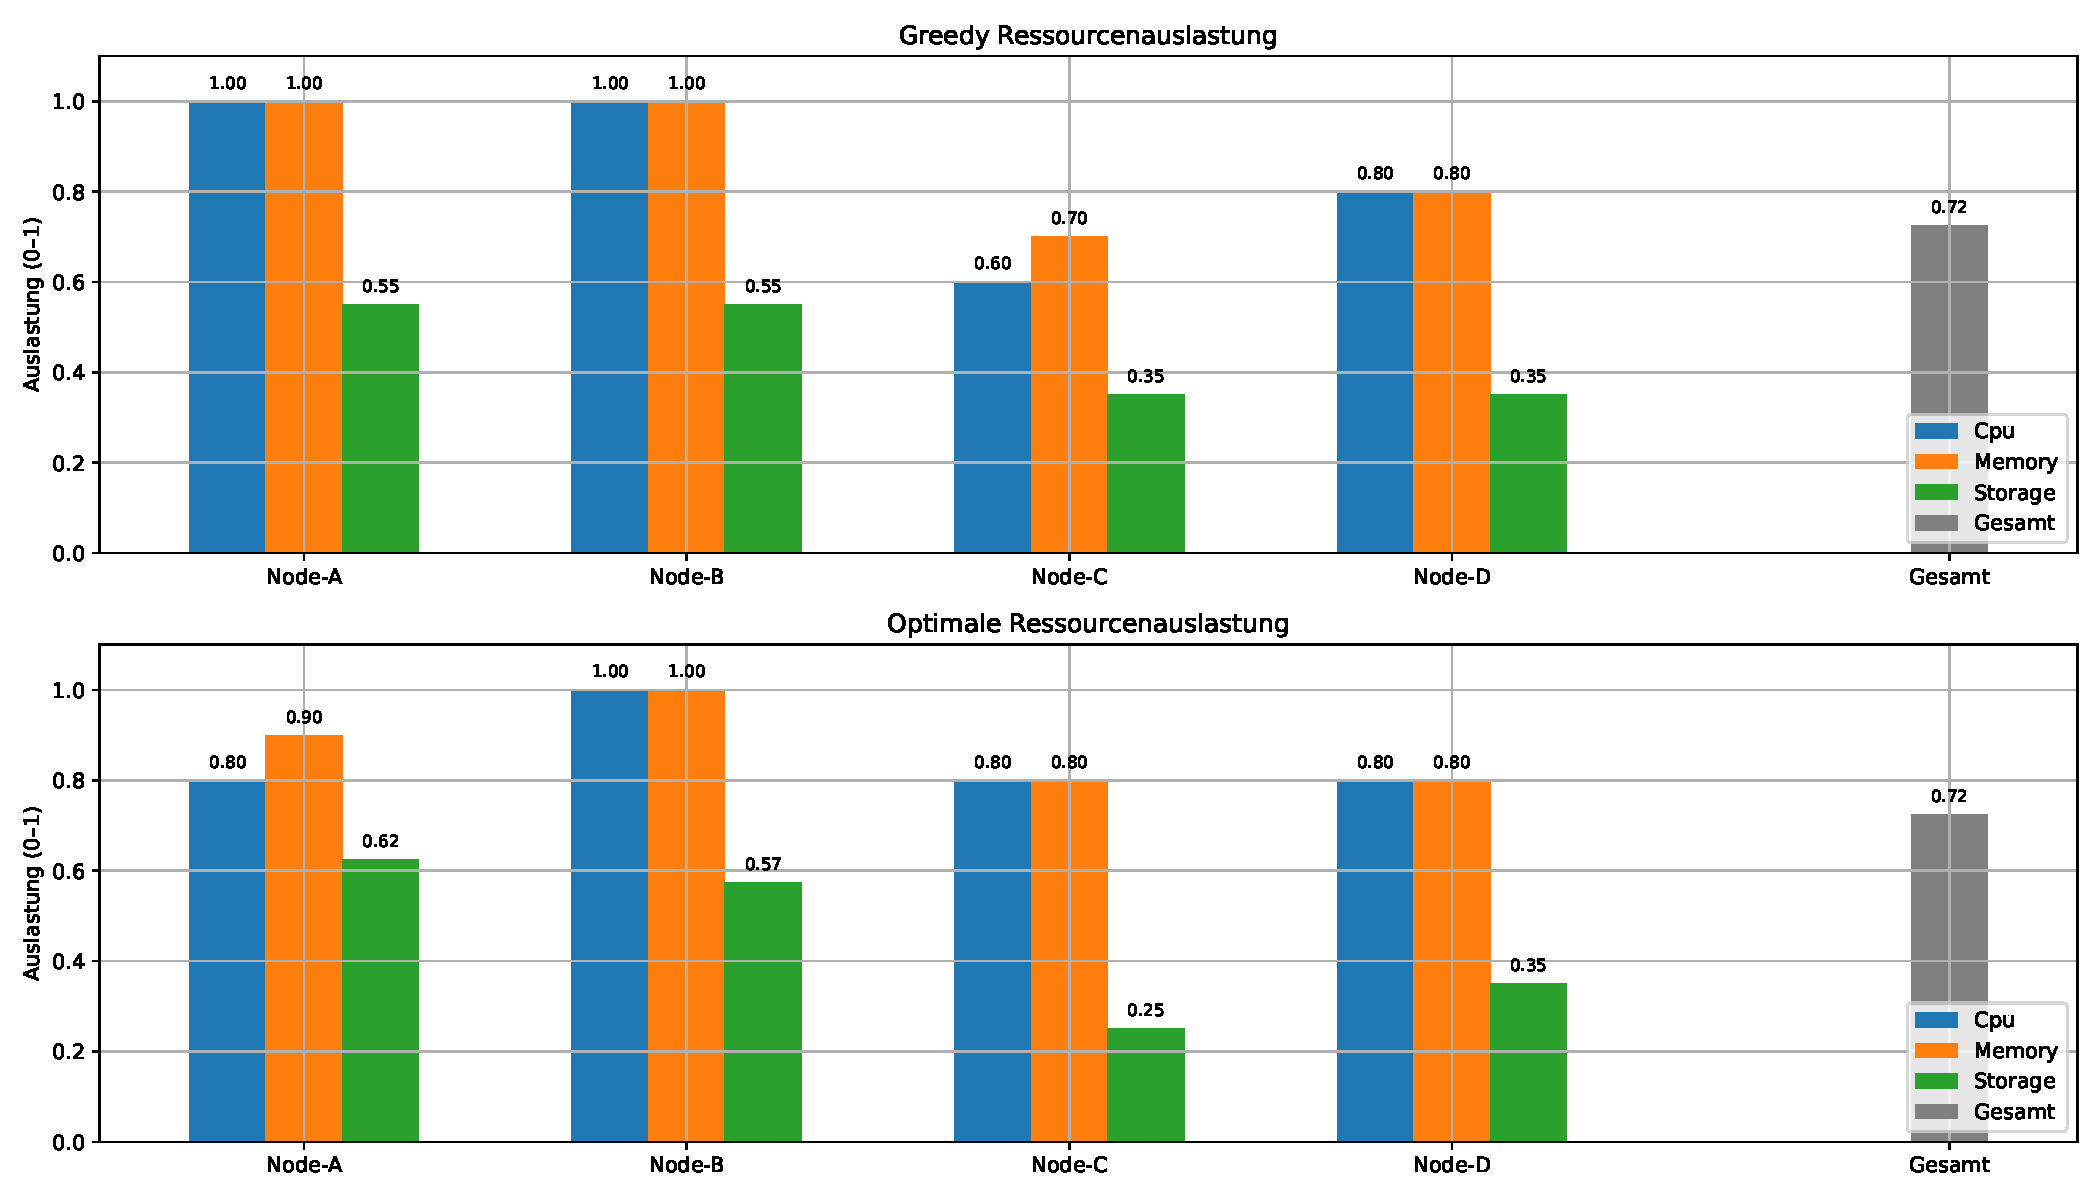
\includegraphics[width=1\textwidth]{./content/graphics/Greedy_vs_Optimal.pdf}
	\caption{Auslastungsvergleich Brute Force und Geedy Scheduling}
	\label{Auslastungsvergleich}
\end{figure}